\chapter{Miami University Simulation Environment (MUSE)}
The implementation and assessment of the different data structures was conducted using our parallel simulation framework called MUSE. The application was developed as part of a master's thesis written by Meseret Gebre in the Department of Computer Science at Miami University in 2009~\cite{gebre-2009}. MUSE was developed in C++ and uses the Message Passing Interface (MPI) library for parallel processing. It also uses Time Warp and standard state saving approach to accomplish optimistic synchronization of the LPs to maintain causality in event processing.

\begin{figure}[!tbp]
\centering
\begin{minipage}[b]{0.75\textwidth}
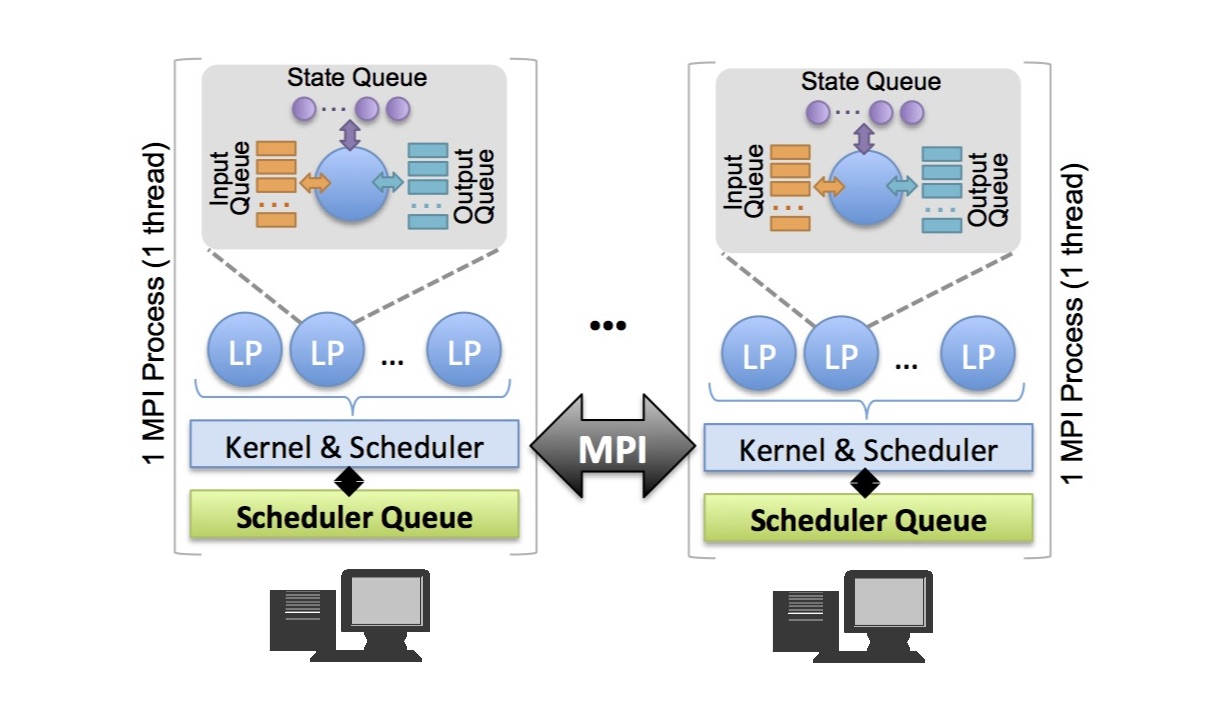
\includegraphics[width=\textwidth]{MUSEarch.jpg}
\textbf{\caption{Overview of a parallel MUSE simulation}}
\label{fig:seesoft}
\end{minipage}
\end{figure}

A conceptual overview of a parallel simulation is shown in Figure~\ref{fig:seesoft}. The simulation kernel implements core functionality associated with LP registration, event processing, state saving, synchronization and Global Virtual Time (GVT) garbage based collection. Each LP in a simulation maintains an input, output and state queue. The input queue is used to handle pending events that have yet to be processed. The output queue stores anti-messages, which are events that are sent to other LPs to cancel out previously sent events. The state queue stores the state of the LP at each discrete point in virtual simulation time. A Time Warp LP also maintains a local virtual time (LVT) that is updated to the time-stamp of the event most recently processed by the LP. 

In a Time Warp based simulation such as MUSE, the simulation is organized as a set of LPs that interact with each other by exchanging virtual times-tamped events. LPs process events in non-decreasing receive-time order and generate new events that are transmitted to LPs on local or remote processors. Synchronization of event processing is achieved through the adherence to the local causality constraint, which requires that LPs only process events in Least Time-stamp First (LTSF) order~\cite{jafer-13}. This is in contrast to the conservative synchronization protocol that blocks event processing until it is guaranteed that an LP cannot receive a future event with a receive-time lesser than it's LVT (altogether avoiding the manifestation of causality errors)~\cite{jafer-13}.

A singular advantage of the Time Warp approach in parallel simulations is the ability to withstand violations of the causality constraint. Time Warp LPs proceed optimistically with event processing and during occasions that an LP encounters an event (\textit{named a \textbf{straggler}}) with a receive time lesser than the LVT, a rollback operation is performed. A rollback requires that an LP undo all event processing that occurred at the LVT equal to the straggler time stamp and forward. The LP performs a rollback to a state with an LVT preceding the straggler time stamp and it sends an anti-message to all other agents with the purpose of cancelling the previously sent events.

As shown in Figure ~\ref{fig:seesoft}, the kernel also maintains a centralized LTSF scheduler queue for managing pending events and scheduling event processing for local LPs. LPs are permitted to generate events only into the future --\textit{i.e.,} the time stamp on events must be greater than their Local Virtual Time (LVT). Consequently, with a centralized LTSF scheduler, event exchanges between local LPs cannot cause rollbacks. Only events received via MPI can cause rollbacks in our simulation. The scheduler is designed to permit different data structures to be used for managing pending events. This feature is used to experiment with the different pending event scheduler queues discussed in the subsequent chapter. A scheduler queue is required to implement the following key operations to manage pending events:

\begin{itemize}
\item[\ding{182}] \textbf{Enqueue one or more future events}: This operation adds the given set of events to the pending event set. Multiple events are added to reprocess events after a rollback.	 

\item[\ding{183}] \textbf{Peek next event}: This operation is expected to return the next event to be processed.  This information is used to determine next LP and to update its LVT prior to event processing. Note that peek does not dequeue events.

\item[\ding{184}] \textbf{Dequeue events for next LP}: In contrast to peek, this operation is expected to dequeue the events to be dispatched for processing by an LP. This operation is performed by the kernel immediately after a peek operation. The operation must dequeue the next set of concurrent events, \textit{i.e.,} events with the same receive time sent to an LP. However, the concurrent events could have been sent by different LPs on different MPI-processes.
Dispatching concurrent events in a single batch streamlines modeling broad range of scenarios. An total order within concurrent events is not imposed but can be readily introduced if needed.	

\item[\ding{185}] \textbf{Cancel pending events}: This operation is used as part of rollback recovery process to aggressively remove \emph{all pending events} sent by a given LP (LP\textsubscript{sender}) to another LP (LP\textsubscript{dest}) at-or-after a given time ($t_{rollback}$). In our implementation, only one anti-message with send time $t_{rollback}$ is dispatched to LP\textsubscript{dest} from LP\textsubscript{sender} to cancel prior events sent by LP\textsubscript{sender} to LP\textsubscript{dest} at-or-after $t_{rollback}$. This is a contrast to conventional aggressive cancellation in which one anti-message is generated per event. This feature short circuits the need to send a large number of anti-messages thereby enabling faster rollback recovery. This feature also reduces scans required to cancel events in Ladder Queue data structures. Note that this feature is reliant on the First-In-First-Out (FIFO) communication guarantee provided by MPI.
\end{itemize}   

\section{Performance Metrics}
As previously stated, we compared the effectiveness of our various PES structures to include the novel structures (\textbf{2tLadderQ} and \textbf{3tHeap}) against the fine-tuned version of the Ladder Queue. The assessment of the data structures involved the following metrics: 
\begin{itemize}
\item[\ding{182}] \textbf{Raw execution run time}: This is the elapsed time between the start and the end of program execution. In a parallel program, the elapse time requires the end time of the last process to finish program execution. Serial and parallel wall clock timings were collected and used in the performance analysis of the various data structures.
\item[\ding{186}] \textbf{Peak Memory Usage}: The total memory used by a serial or parallel program.
\item[\ding{187}] \textbf{Cache Hits or Misses}: Number of times that accessed data is found or not found to reside in cache memory.
\end{itemize}

\section{Experimental Platform}~\label{sec:platform}
The design of MUSE and the experiments reported were conducted using a distributed-memory compute cluster consisting of 80 compute nodes interconnected by 1 GBPS Ethernet. Each compute node has 8 cores from two quad-core Intel Xeon \textregistered CPUs (E5520) running at 2.27 GHz with hyper-threading disabled. Each compute node has 32 GB of RAM (4 GB per core) in Non-Uniform Memory Access (NUMA) configuration. The cluster has an independent 1 GBPS Ethernet network to support a shared file system. The nodes run Red Hat Enterprise Linux 6, with Linux (kernel ver 2.6.32) and the cluster runs PBS/Torque. The simulation software was compiled using GCC version 4.9.2 (\textbf{-O3} optimization) with OpenMPI 1.6.4. All debug assertions were turned off for maximum performance.
